\chapter{Optimizing network-utilization by balancing workload}
\label{chap:balancing}

The last chapter brings an overview of different notations, algorithms and techniques.
In this chapter, all these instruments are combined to a chain for distributing routes more evenly.
The goal is to augment a given graph, such that diverse alternative paths can be found and used to spread too much load while limiting the detours of individual \glspl{stpair}.
After the theory is explained, implementation-details are discussed.
When talking about performance, it is referred to the used testing-machine, which is an ordinary, but good home-computer.
Further details about the testing-machine and experimental results can be found in \vref{chap:experiments}.

For a given \gls{stpair} and a graph $G = (V, E)$ with vertices $V$ and edges $E$ of multidimensional \glspl{weight}, a path should be found through an algorithm, that implicitly tends to distribute found paths over the network, while keeping the paths' \glspl{cost} sufficiently near every \gls{cost}-dimension's optimum.
To achieve this, a computation-phase called \gls{balancing} analyzes the graph $G$ and computes a new \gls{metric}, called workload-\gls{metric}.
With this workload-\gls{metric}, routing-algorithms like \gls{repr} and \gls{dijkstra} (with \gls{personalized_routing}) can compute paths as usual.
For comparison, multiple scenarios using different combinations of these two routing-algorithms will be used.
Please note, that \gls{dijkstra} doesn't guarantee a tolerance when used with \gls{personalized_routing} and hence, some combinations don't provide an upper bound for path-costs.
This will also be pointed out in the respective experiments in \vref{chap:experiments}.

This thesis focusses only on distance and travel-time, where travel-time is the only \gls{metric} with a provided tolerance.

It should be noted, that \gls{dijkstra} (bidirectional) instead of \gls{astar} is used for every occuring routing-query, may it be in \gls{repr} or anywhere else.
The reason is, that \gls{astar} works with heuristics, which are difficult to generalize over custom, artificial \glspl{metric}.
The only benefit from using \gls{astar} is the reduction of the search-space, which can be reduced much more using bidirectional \gls{dijkstra} on graphs contracted via \gls{contraction-hierarchies}.
Besides that, the graph has multidimensional \glspl{metric}, for which reason \gls{dijkstra} is used with \gls{personalized_routing}.

\section{Balancing to create a new metric}

    \todo{both approaches: multiple runs (explicit euler because workload is toggling) vs multiple workload-\glspl{metric}}

    This \gls{balancing} is depicted in \vref{fig:balancing} and explained briefly in the caption or detailled in the following.

    \begin{figure}
        \centering
        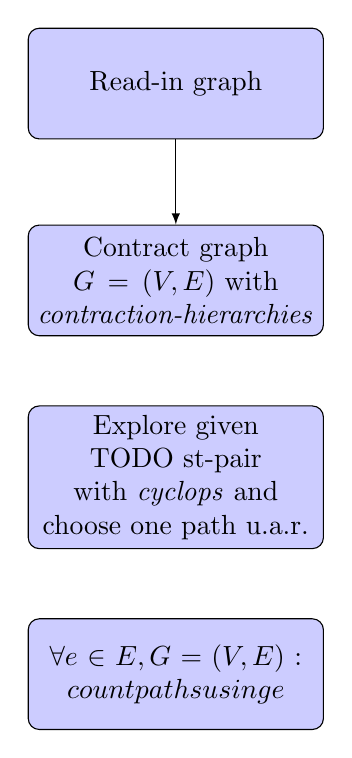
\begin{tikzpicture}[auto, rounded corners=0, node distance = 3cm, x=1cm, y=1cm] {%
    % style

    % draw
    % Draw borders

    % text badly centered
    % better use 'align=flush center'

    \tikzstyle{decision} = [%
        diamond,
        draw,
        fill = blue!20,
        text width = 4.5em,
        align = flush center,
        node distance = 3cm,
        inner sep = 0pt
    ]
    \tikzstyle{block} = [%
        rectangle,
        draw,
        fill = blue!20,
        text width = 10em,
        text centered,
        rounded corners,
        node distance = 2.5cm,
        minimum height = 4em
    ]
    \tikzstyle{cloud} = [%
        draw,
        ellipse,
        fill = red!20,
        node distance = 3cm,
        minimum height = 2em
    ]

    % arrow-styles
    % https://tex.stackexchange.com/questions/5461/is-it-possible-to-change-the-size-of-an-arrowhead-in-tikz-pgf
    \tikzstyle{line} = [draw, -latex]

    % Place nodes

    \node [block] (read-in_graph) {Read-in graph};
    \node [block, below of = read-in_graph] (contract_graph) {Contract graph $G=(V,E)$ with \textit{contraction-hierarchies}};
    \node [block, below of = contract_graph] (exploration) {Explore given TODO st-pair with \textit{cyclops} and choose one path u.a.r.};
    \node [block, below of = exploration] (analyzation) {$\forall e \in E, G = (V, E): count paths using e$};

    % Draw lines

    \path [line] (read-in_graph) -- (contract_graph);

    % \node [block] (init) {initialize model};
    % \node [cloud, left of=init] (expert) {expert};
    % \node [cloud, right of=init] (system) {system};

    % \node [block, below of=init] (identify) {identify candidate models};

    % \node [block, below of=identify] (evaluate) {evaluate candidate models};
    % \node [block, left of=evaluate, node distance=3cm] (update) {update model};

    % \node [decision, below of=evaluate] (decide) {is best candidate better?};

    % \node [block, below of=decide, node distance=3cm] (stop) {stop};

    % % Draw edges

    % \path [line] (init) -- (identify);
    % \path [line] (identify) -- (evaluate);
    % \path [line] (evaluate) -- (decide);
    % \path [line] (decide) -- node {no} (stop);

    % \path [line] (update) |- (identify);
    % \path [line] (decide) -| node [near start] {yes} (update);

    % \path [line,dashed] (expert) -- (init);
    % \path [line,dashed] (system) -- (init);
    % \path [line,dashed] (system) |- (evaluate);
} \end{tikzpicture}
        \caption[Overview of balancing a graph]{%
            This flow shows the \gls{balancing}, that analyzes a given graph $G$.
            Here, an evaluation-phase is included afterwards.
            Shapes for actions are rectangular and blue, shapes for data are elliptical and red.
            A new, artificial \gls{metric} is created for $G$ and gets updated iteratively.
            In the end, this new \gls{metric} allows a routing-algorithm to distribute upcoming workload (like during rush-hour) more evenly over the underlying street-network in $G$.
            This more spreaded workload can be seen in the evaluation-step, where paths for a set of \glspl{stpair} are searched, once using and once ignoring the new metric.

            Note, that the path-search ignores the new \gls{metric} in the first iteration.
            \label{fig:balancing}
        }
    \end{figure}

    \subsection{Selection of route-pairs}

        \todo{TODO @Florian: Opinion about how following Absatz is written?}
        Let a street-network be given as a graph $G = (V, E)$ of multidimensional \glspl{metric}.
        For simplicity, the set of \glspl{stpair}, which is used for balancing $G$, consists of $s$ and $t$ chosen \gls{uar}\ from $V$.
        This has the disadvantage, that a sufficiently large set of \glspl{stpair} is needed to overload $G$.
        This clearly becomes a bottleneck for performance on larger graphs (beginning with small German states like Saarland with almost $|V| \approx \num{580000}$ and $|E| \approx \num{1160000}$ after parsing), especially when using \gls{repr}, that computes multiple \gls{dijkstra}-queries per run.
        On the other side, real, daily, critical \glspl{stpair} are not distributed \gls{uar}\ over $V$.
        The rush-hour in the morning, when everybody travels from their home to work, is a good counterexample here.
        The set of chosen $t$ might be much smaller than the number of $s$, and less people live near industry or motorways.
        Heuristics as described in~\cite{bakillah:population_from_osm} can return \glspl{stpair} based on approximating population-data from street-networks.
        So considering more specific sets of \glspl{stpair} might be interesting and helpful to boost the \gls{balancing} up, but is not covered in this thesis.
        The reason for keeping the choice \gls{uar}\ is the easy implementation, while results are sufficiently good enough, as long as $G$ shows overloaded streets.

    \subsection{First steps of the balancing-process}

        At first, the graph $G$, that should be balanced, has to be read in.
        Before continuing, every \gls{metric} is divided by the respective \gls{metric}-mean resulting in $G = (V, E)$ of normalized \glspl{metric}.
        Non-normalized \glspl{metric} of different scales would cause \gls{repr} to find $\alpha$-values of different scale, making some \glspl{metric} more important than others just based on their different scales.
        With \glspl{metric} of different importance, the chosen paths tend to the respective \glspl{metric} and distort the spread.
        So normalization doesn't just allow to compare different graphs, but also improves the spread in \gls{repr}.

        This graph $G$ is contracted via \gls{contraction-hierarchies} to $G_{CH}$.
        The step of contracting is not needed for correctness, but reduces the needed runtime (even if $G$ is not being fully contracted).

        Given the \glspl{stpair} and $G_{CH}$, a path in $G_{CH}$ is searched for every \gls{stpair}.
        The search may use either \gls{dijkstra} or \gls{repr}.
        Multiple paths are found by \gls{repr}, so one of them is chosen \gls{uar}\ after filtering all found paths by a given tolerance.
        Note, that \gls{dijkstra} with \gls{personalized_routing} doesn't consider any tolerance.
        But since \gls{repr} calls \gls{dijkstra} multiple times, just \gls{dijkstra} is faster.
        On the other hand, when using \gls{repr} with choosing a path \gls{uar}, the resulting paths are more spreaded over the network.
        This results in a better coverage of $E$ when updating the workload-\gls{metric}, which allows the \gls{repr} to find more pareto-optimal \glspl{personalized_route} in the convex-hull.
        Both methods are compared in the experiments in \vref{chap:experiments}.

        When using \gls{repr}, the quality of the balanced graph highly depends on the choice of initial paths for \gls{repr}.
        The basic approach in~\cite{barth:alternative_multicriteria_routes} suggests to use $(d+1)$ initial alphas to define the initial convex-hull for a graph of $d$-dimensional \glspl{metric}.
        \begin{equation}
        \begin{aligned}
            \left( \alpha^{(1)}, \alpha^{(2)}, \dots, \alpha^{(d)} \right) &= \mathbb{I}^d\\
            \alpha^{(d+1)} &= \left( \frac{1}{d} \right)_{i = 1,\dots, d}
        \end{aligned}
        \end{equation}
        This suggestion doesn't work well for the \gls{balancing}.
        When the new workload-\gls{metric} is added (hence let the graph's \glspl{metric}' dimension be $d+1$), $\alpha^{(d+1)}$ becomes $\alpha^{(d+2)}$, which is a different direction in the $(d+1)$-cost-space than the previous $\alpha^{(d+1)}$ points to in the $(d+1)$-cost-space.
        Because of this, less paths have been found on Saarland in the experiments.
        Especially when talking in general, the first iteration may find paths, that can't be found by latter iterations.
        Therefore, the \gls{balancing} extends the original suggestion by~\cite{barth:alternative_multicriteria_routes} and takes the initial $\alpha^{(j)}$ from the $(d+1)$-dimensional power-set of $(1, \dots, 1)^T$ without $(0, \dots, 0)^T$.
        Only the direction of $\alpha$ is relevant, so the previous notation can be simplified.
        \begin{equation}
            \label{eq:new_init_alphas}
            \alpha \in \left\{ 0, 1 \right\}^{(d+1)} \setminus \left\{ \left( 0, \dots, 0 \right)^T \right\} \Rightarrow \alpha \text{ is an initial } \alpha^{(j)}
        \end{equation}

        After finding a set of paths for the given \glspl{stpair}, every edge counts the number of found paths using the counting edge.
        This workload of \gls{balancing}-iteration $i$ is normalized by all workloads' mean and the result is used to update the graph's workload-\gls{metric}.
        \begin{equation}
        \label{eq:workloads}
        \begin{aligned}
            &\mathit{workloads}_i = \left\{ \left| \left\{ \mathit{path}_{s,t} : \mathit{path}_{s,t} \text{ uses } e \right\} \right| : \forall e \in E_{CH} \right\}\\
            \Rightarrow\ &\mathit{new}_i = \frac{\mathit{workloads}_i}{\mathit{mean}(\mathit{workloads}_i)}
        \end{aligned}
        \end{equation}

    \subsection{Updating the new metric with the collected workload}

        Updating the old workload-\gls{metric} is a very small step in the \gls{balancing} with a large impact on the ongoing \gls{balancing}'s performance and the quality of the balanced graph.
        Two approaches have been tested and are depicted in the following.
        \todo{%
            TODO @Florian next sentence with \quotes{first approach, second approach}. Your opinion about the language (\eg\ \quotes{as wished})?
        }
        The first approach (see \vref{eq:euler}) is kind of a failing first try, whereas the second one (see \vref{eq:averaging}) is working well, as wished.

        The workload-\gls{metric} can be associated with popularity, because it refers to high usage.
        A path of high popularity should be chosen less often than without the workload-\gls{metric}.
        So, hopefully, updating the workload-\gls{metric} dependent on the current workload-\gls{metric} reveals the final, balanced state of the network eventually.
        You could argue, that a street's capacity should be considered as well, because large streets like motorways can support more vehicles than a street in a city.
        A street-capacity could be approximated using a street's number of lanes or the respective street-type (\eg\ motorways) and its length.
        Herewith, the workload-\gls{metric}, penalizing popularity, would be corrected in favor of larger streets with (usually) higher speed-limit.
        That is exactly contraproductive, because the travel-time does already consider the capacity of streets with the speed-limit.
        In other words, the popularity-penalization should compensate the popularity of larger streets with better travel-time.
        This wished effect would be disturbed by the consideration of capacity.

        The first approach is inspired by a simpler numerical method for solving initial-value-problems called \gls{explicit_euler}.
        Let $\mathit{old}_i$ be the workload-\gls{metric} (already normalized after $G$ has been initialized) already stored in the graph and $\mathit{new}_i$ the new workload-\gls{metric} (normalized by new mean, see \vref{eq:workloads}).
        \begin{equation}
        \label{eq:euler}
            \mathit{old}_{i+1} = \mathit{old}_i + (\mathit{new}_i - \mathit{old}_i) \cdot \mathit{correction}
        \end{equation}
        In each \gls{balancing}-iteration, after the workload-\gls{metric} is updated (as in \vref{eq:euler}), every value of the workload-\gls{metric} smaller than a predefined minimum value $\epsilon$ (\eg\ \num{0.1}) is set to $\epsilon$.
        This removes the \glspl{metric} of value \num{0.0}, which improves the set of computed shortcuts when applying \gls{contraction-hierarchies} and thus performance.
        In addition, the result isn't normalized by its mean in general, for which reason it is finally normalized.
        \begin{equation}
        \label{eq:metric_cleanup}
        \begin{aligned}
            \mathit{old}_{i+1} &= \mathit{max} \left( \epsilon \text{,\ } \mathit{old}_{i+1} \right)\\
            \mathit{old}_{i+1} &= \frac{\mathit{old}_{i+1}}{\mathit{mean}(\mathit{old}_{i+1})}
        \end{aligned}
        \end{equation}

        In fact, this approach works okay in smaller, overloaded networks like Isle~of~Man ($|V| \approx \num{50000}$ and $|E| \approx \num{100000}$ after parsing), but lacks in convergence.
        In the first update-iteration, popular paths are ignored as much as possible, before they are highly preferred in the second iteration, ignored in the third iteration and so on.
        This behaviour could be reduced by adding the $\mathit{correction}$, but larger networks (like the small German state Saarland, $|V| \approx \num{580000}$ and $|E| \approx \num{1160000}$ after parsing) worsen the convergence.

        Therefore, another approach, replacing the \gls{explicit_euler} from \vref{eq:euler}, is presented in the following, that does spread the workload well and within only two iterations.
        \begin{equation}
        \label{eq:averaging}
            \mathit{old}_{i+1} = \frac{i \cdot \mathit{old}_i + \mathit{new}_i}{i+1}
        \end{equation}
        This result is treated as before, meaning \vref{eq:metric_cleanup} are also applied.
        From \vref{eq:averaging}, both $\mathit{old}_1=\mathit{new}_0$ and $\mathit{old}_2=\frac{\mathit{old}_1 + \mathit{new}_1}{2}$ hold before normalization.
        The interpretation of these is quite intuitive.
        The first iteration favors popular routes.
        After the first update, the workload-\gls{metric} is just the normalized workload from the original, unbalanced graph.
        Hence the following iteration has an aversion to popular routes and tends to avoid them.
        This second iteration favors alternative routes and the outcoming workload completes the previously generated workload-\gls{metric} evenly weighted.
        A third iteration has already a workload-\gls{metric} with a balance between popular and alternative routes, so further iterations appear disruptive.

\section{Evaluating the balanced graph by executing queries}

    \todo{%
        TODO

        Queries can be done via \gls{dijkstra} or \gls{repr}.
    }

    \todo{%
        TODO

        Evaluation with \glspl{stpair}, that differ from those, that are used for optimization!\\
        $\Rightarrow$ training-\glspl{stpair} vs evaluation-\glspl{stpair}
    }

\section{Some theoretical implementation-details}
\label{chap:balancing:implementation}

    \todo{highlights, what was difficult/much work? -> repo-link}

    \subsection{Graphs and paths}

        \todo{TODO Write: Street-network as offset-graph (TODO: wrong name)}

        \todo{TODO Accessing the graph-structure}

    \subsection{Configs}

        \todo{TODO add some text here}
% - indices -> boost for performance while staying dynamic
% - Dijkstra, no A* because multiple metrics vs heuristic